\chapter{Deep Generation Model}

\begin{itemize}
    \item \textbf{Generative} models can capture the joint probability $p(X, Y)$, or just $p(X)$ if there are no labels
    \item \textbf{Discriminative} models capture the conditional probability $p(Y|X)$
\end{itemize}

How can we generate new data instances? If we had the data distribution $p(X)$, we could just sample
from it and then we would get all the instances.
\begin{equation}
    \begin{split}
        p(\mathbf{z}, \mathbf{x}) = p(\mathbf{z})p(\mathbf{x}|\mathbf{z}) = p(\mathbf{x})p(\mathbf{z}|\mathbf{x})
    \end{split}
\end{equation}
\begin{equation}
    \begin{split}
        p(\mathbf{z}|\mathbf{x}) = \frac{p(\mathbf{z}, \mathbf{x})}{p(\mathbf{x})}
        = \frac{p(\mathbf{z})p(\mathbf{x}|\mathbf{z})}{p(\mathbf{x})}
    \end{split}
\end{equation}
\begin{equation}
    \begin{split}
        p(\mathbf{x}) = \int p(\mathbf{z})p(\mathbf{x}|\mathbf{z})d \mathbf{x}
    \end{split}
\end{equation}

函数的函数是泛函
求泛函的极值方法是变分法

\section{Variational Inference}

Consider a joint density of latent variables $\mathbf{z}$ and observations $\mathbf{x}$
\begin{equation}
    p(\mathbf{z}, \mathbf{x}) = p(\mathbf{z})p(\mathbf{x}|\mathbf{z})
\end{equation}

In Bayesian models, the latent variables help govern the distribution of the data. A Bayesian
model draws the latent variables from a \textbf{prior density $p(\mathbf{z})$} and then relates them to the
observations through the \textbf{likelihood $p(\mathbf{x} | \mathbf{z})$}. Inference in a Bayesian model amounts to
conditioning on data and computing the \textbf{posterior $p(\mathbf{z} | \mathbf{x})$}. In complex Bayesian models,
this computation often requires approximate inference.

The main idea behind variational inference is to use optimization. Variational inference thus turns the
inference problem into an optimization problem
First, we posit a family of approximate densities Q. This is a set of densities over the latent
variables. Then, we try to find the member of that family that minimizes the Kullback-Leibler
(KL) divergence to the exact posterior,
\begin{equation}
    q^*(\mathbf{z}) = \arg \min_{q(\mathbf{z}) \in \mathcal{Q}} KL(q(\mathbf{z}) \| p(\mathbf{z}|\mathbf{x}))
\end{equation}
Finally, we approximate the posterior with the optimized member of the family $q^*(\mathbf{z})$

\begin{equation}
    \begin{split}
        KL(q(\mathbf{z})\|p(\mathbf{z}|\mathbf{x}))
        &= \mathbb{E}_{q(\mathbf{z})} [\log q(\mathbf{z})] - \mathbb{E}_{q(\mathbf{z})} [\log p(\mathbf{z}|\mathbf{x})] \\
        &= \mathbb{E}_{q(\mathbf{z})} [\log q(\mathbf{z})] - \mathbb{E}_{q(\mathbf{z})} [\log p(\mathbf{z}, \mathbf{x})] + \mathbb{E}_{q(\mathbf{z})}[\log p(\mathbf{x})]\\
        &= \mathbb{E}_{q(\mathbf{z})} [\log q(\mathbf{z})] - \mathbb{E}_{q(\mathbf{z})} [\log p(\mathbf{z}, \mathbf{x})] + \log p(\mathbf{x}) \\
        \\
        \log p(\mathbf{x})
        &= KL(q(\mathbf{z})\|p(\mathbf{z}|\mathbf{x})) + \mathbb{E}_{q(\mathbf{z})} [\log p(\mathbf{z}, \mathbf{x})] - \mathbb{E}_{q(\mathbf{z})} [\log q(\mathbf{z})]
    \end{split}
\end{equation}

$\log p(\mathbf{x})$ is constant with respect to $q(\mathbf{z})$, $KL(\cdot ) \ge 0$, then
\begin{equation}
    ELBO(q) = \mathbb{E}_{q(\mathbf{z})} [\log p(\mathbf{z}, \mathbf{x})] - \mathbb{E}_{q(\mathbf{z})} [\log q(\mathbf{z})]\le \log p(\mathbf{x})
\end{equation}

The function is call \textbf{evdience low bound(ELBO)}. Maximizing the ELBO is equivalent to
minimizing the KL divergence.

\begin{equation}
    \begin{split}
        ELBO(q)
        &= \mathbb{E}_{q(\mathbf{z})} [\log p(\mathbf{z}, \mathbf{x})] - \mathbb{E}_{q(\mathbf{z})} [\log q(\mathbf{z})] \\
        &= \mathbb{E}_{q(\mathbf{z})} [\log p(\mathbf{z})] + \mathbb{E}_{q(\mathbf{z})} [\log p(\mathbf{x}|\mathbf{z})] - \mathbb{E}_{q(\mathbf{z})} [\log q(\mathbf{z})] \\
        &= \mathbb{E}_{q(\mathbf{z})} [\log p(\mathbf{x} | \mathbf{z})] - KL(q(\mathbf{z})\|p(\mathbf{z}))
    \end{split}
\end{equation}

The first termis an expected likelihood; it encourages densities
that place their mass on configurations of the latent variables
that explain the observed data. The second term is the negative
divergence between the variational density and the prior; it encourages
densities close to the prior.

\subsection{Regularizer - Solution of $- KL(q(\mathbf{z})\|p(\mathbf{z}))$, Gaussion case}
\begin{quotation}
    VAEs take an unusual approach to dealing with this problem: they assume that there is no simple interpretation
    of the dimensions of z, and instead assert that samples of z can be drawn from a simple distribution, i.e.,
    $\mathcal{N}(0, I)$, where $I$ is the identity matrix. The key is to notice that any distribution in $d$ dimensions 
    can be generated by taking a set of $d$ variables that are normally distributed and mapping them through a sufficiently 
    complicated function.
\end{quotation}

When both prior $p_{\mathbf{\theta}}(z) = N(0; I)$ and the posterior
approximation $q_{\phi}(z|x^{(i)})$ are Gaussian. Let
$J$ be the dimensionality of $\mathbf{z}$. Let $\mathbf{\mu}$ and $\mathbf{\sigma}$ denote the
variational mean and s.d. evaluated at datapoint $i$, and let $\mu_j$ and
$\sigma_j$ simply denote the $j$-th element of these vectors. Then

\begin{equation}
    \begin{split}
        \int q_{\mathbf{\theta}}(\mathbf{z}) \log p(\mathbf{z}) d\mathbf{z}
        &= \int \mathcal{N}(\mathbf{z}; \mathbf{\mu}, \mathbf{\sigma}^2) \log \mathcal{N}(\mathbf{z}; \mathbf{0}, \mathbf{I}) d \mathbf{z} \\
        &= -\frac{J}{2} \log (2\pi) -\frac{1}{2} \sum^J_{j=1}(\mu^2_j + \sigma^2_j)
    \end{split}
\end{equation}

And:

\begin{equation}
    \begin{split}
        \int q_{\mathbf{\theta}}(\mathbf{z}) \log q_{\mathbf{\theta}}(\mathbf{z}) d \mathbf{z}
        &= \int \mathcal{N}(\mathbf{z}; \mathbf{\mu}, \mathbf{\sigma}^2) \log \mathcal(N)(\mathbf{z}; \mathbf{\mu}, \mathbf{\sigma}^2) d\mathbf{z} \\
        &= -\frac{J}{2} \log (2\pi) - \frac{1}{2} \sum^J_{j=1}(1 + \log \sigma^2_j)
    \end{split}
\end{equation}

Therefore:

\begin{equation}
    \begin{split}
        - KL(q(\mathbf{z})\|p(\mathbf{z})) = \frac{1}{2}\sum^J_{j=1}(1 + \log\sigma_j^2 - \mu_j^2 - \sigma_j^2)
    \end{split}
\end{equation}


\subsection{Reconstruction Error}
The usual choice is to say that $q(z|x) = \mathcal{N}(z| \mu(x; \boldsymbol{\theta}), \Sigma(\mathbf{x}; \boldsymbol{\theta}))$,where
$\mu$ and $\Sigma$ are arbitrary deterministic functions with parameters $\theta$ that can be learned from data. In practice, $\mu$ and $\Sigma$
are again implemented via neural networks, and $\Sigma$ is constrained to be a diagonal matrix.

ELBO可以写为
\begin{equation}
    ELBO(\boldsymbol{\theta}, \phi, \mathbf{x}) 
    = \mathbb{E}_{q_{\phi}(\mathbf{z}|\mathbf{x})} [\log p_{\boldsymbol{\theta}}(\mathbf{x} | \mathbf{z})] 
        - KL(q_{\phi}(\mathbf{z}|\mathbf{x})\|p_{\boldsymbol{\theta}}(\mathbf{z}))
\end{equation}
We want to \textbf{differentiate} and optimize the lower bound $ELBO(\boldsymbol{\theta}, \phi, \mathbf{x})$ w.r.t both the variational
parameters $\phi$ and generativet parameters $\theta$.由于隐变量$z$从$q(z|x)$的采样过程不可微,所以需要改写成一个可微的形式.
we can reparameterize the random variale $z \sim  q_{\phi}(z|x)$ using a differentiable transformation $g_{\phi}(\epsilon, x)$ of an 
(auxiliary) noise variable $\epsilon$
\begin{equation}
    \tilde{\mathbf{z}} = g_{\phi}(\boldsymbol{\epsilon}, \mathbf{x}) \quad with \quad \boldsymbol{\epsilon} \sim p(\boldsymbol{\epsilon})
\end{equation}

\subsection{Reparameterization trick}
Given $\mu(\mathbf{x})$ and $\Sigma(\mathbf{x})$—the mean and covariance of $q(z|x)$ — we can sample from
$\mathcal{N}(\mu(x), \Sigma(x))$ by first sampling $\epsilon \sim \mathcal{N}(0, I)$, then computing 
$z = \mu(x) + \Sigma^{\frac{1}{2}}(x) * \epsilon$.

\begin{figure}[H]
    \centering
    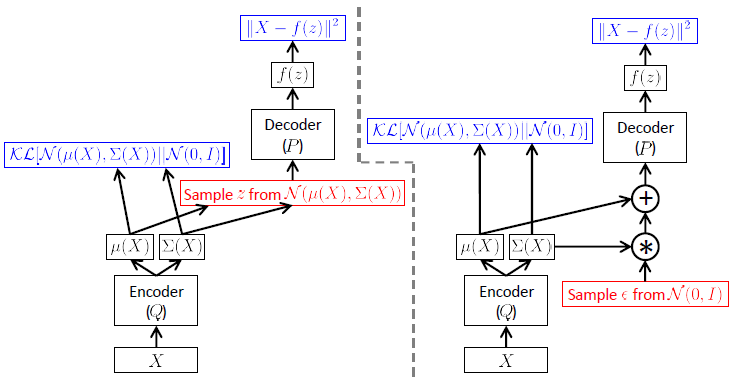
\includegraphics[width=12cm]{images/vae_reparameterization_trick.png}
    \label{fig:vae_reparameterization_trick}
\end{figure}

\section{VAE}
\begin{figure}[H]
    \centering
    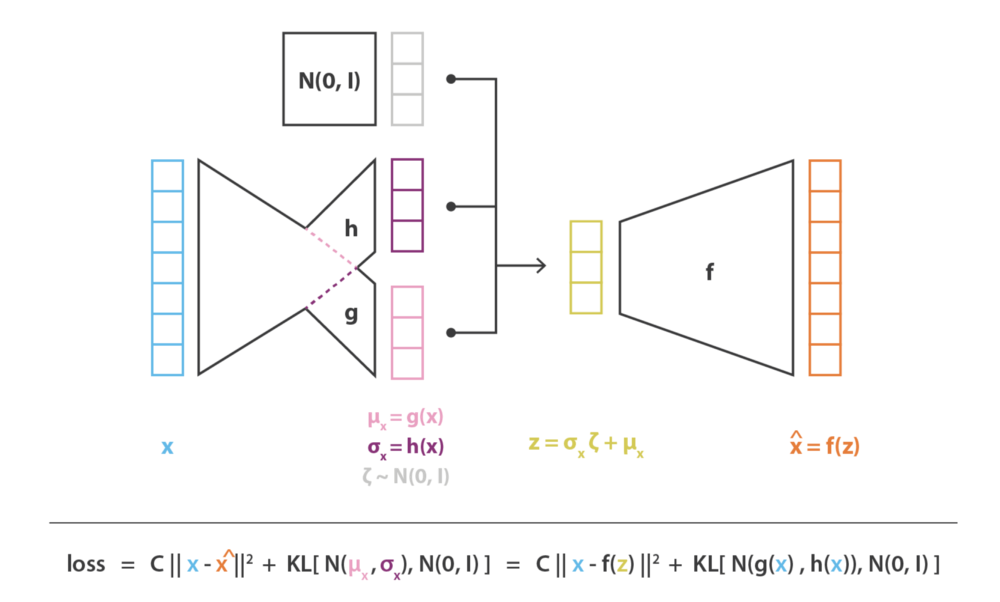
\includegraphics[width=12cm]{images/vae.png}
    \caption{vae}
    \label{fig:VAE}
\end{figure}
\subsection{为什么需要VAE?为什么不直接使用Autoencoder的decoder来生成图片?}

Autoencoder的encoder生成的latent space不够regurlarity(不连续),我们无法从latent space的中随机采样来生成或修改图片
\begin{quotation}
    the lack of interpretable and exploitable structures in the latent space (\textbf{lack of regularity}).
    the regularity of the latent space for autoencoders is a difficult point that depends on the distribution of the data in the initial space, the dimension of the latent space and the architecture of the encoder. So, it is pretty difficult (if not impossible) to ensure, a priori, that the encoder will organize the latent space in a smart way compatible with the generative process we just described.
\end{quotation}
\begin{figure}[H]
    \centering
    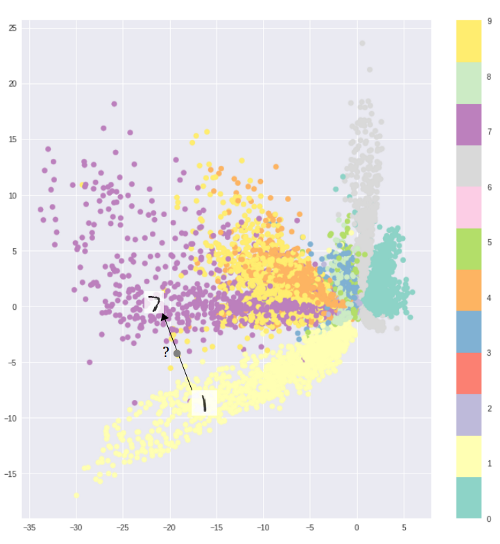
\includegraphics[width=8cm]{images/mnist_ae_latent_space.png}
    \caption{the encodings from a 2D latent space / MNIST}
    \label{fig:mnist_ae_latent_space}
\end{figure}

\subsection{VAE}
\begin{quotation}
    a variational autoencoder can be defined as being an autoencoder whose training is
    regularised to avoid overfitting and ensure that the latent space has good properties
     that enable generative process.
\end{quotation}
VAE模型需要符合以下条件
\begin{itemize}
    \item the input is \textbf{encoded as distribution} over the latent space, instead of encoding an input as a single point
    \item a point from the latent space is sampled from that distribution
    \item the sampled point is decoded and the reconstruction error can be computed
    \item the reconstruction error is backpropagated through the network
\end{itemize}
\begin{figure}[H]
    \centering
    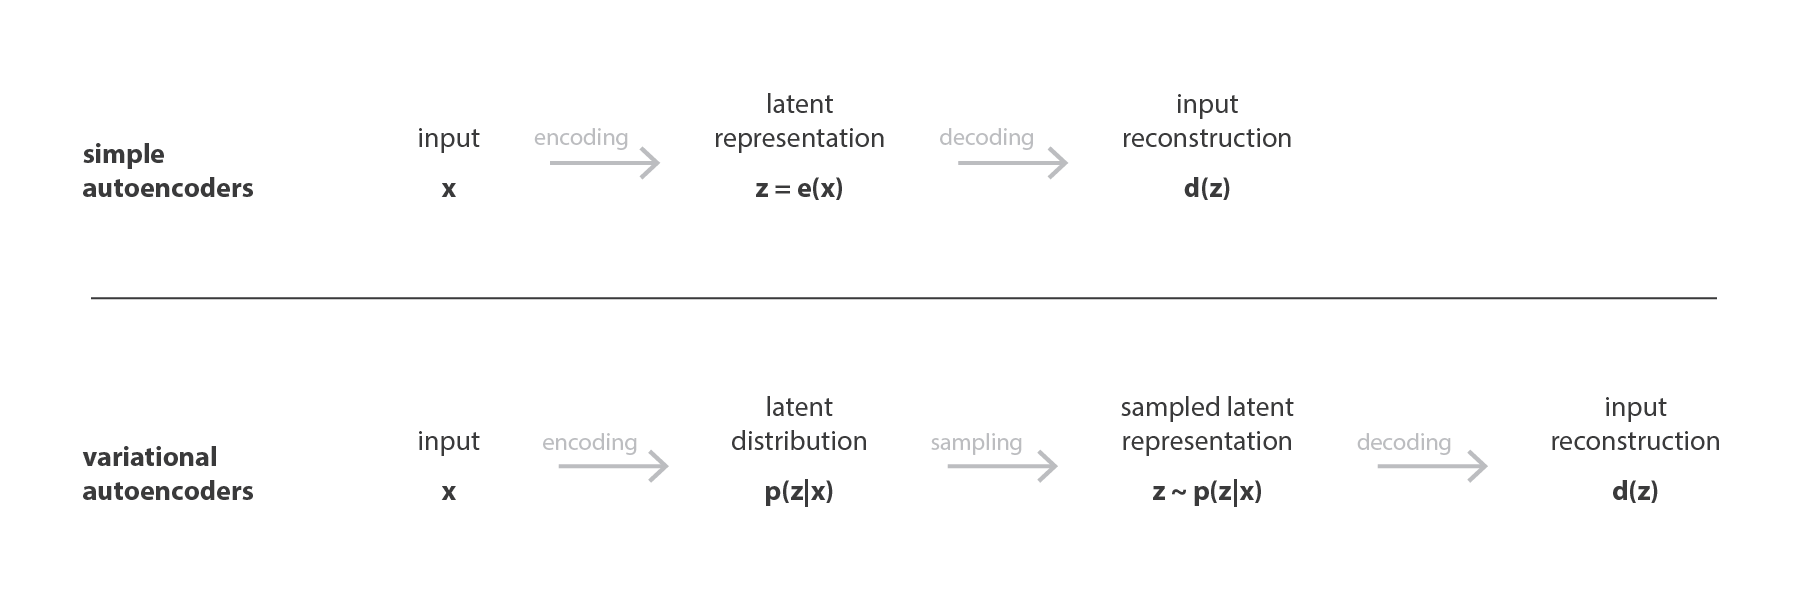
\includegraphics[width=16cm]{images/ae_vae.png}
    \label{fig:AEvsVAE}
\end{figure}

Latent space应该具有以下的性质
\begin{itemize}
    \item \textbf{Continuity} two close points in the latent space should not give two completely different contents once decoded
    \item \textbf{Completeness} for a chosen distribution, a point sampled from the latent space should give “meaningful” content once decoded
\end{itemize}
\begin{figure}[H]
    \centering
    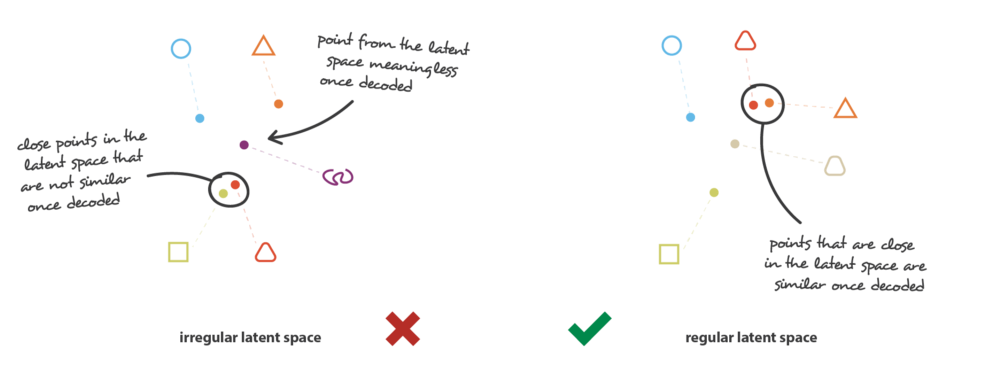
\includegraphics[width=16cm]{images/irregular_latent_space.png}
    \label{fig:irregular_latent_space}
\end{figure}
The only fact that VAEs encode inputs as distributions instead of simple points is
not sufficient to ensure continuity and completeness. Without a well defined
regularisation term, the model can learn, in order to minimise its reconstruction
error, to “ignore” the fact that distributions are returned and behave almost like
classic autoencoders (leading to overfitting). To do so, the encoder can either return
distributions with tiny variances (that would tend to be punctual distributions(点分布)) or return
distributions with very different means (that would then be really far apart from each other
in the latent space).
\begin{figure}[H]
    \centering
    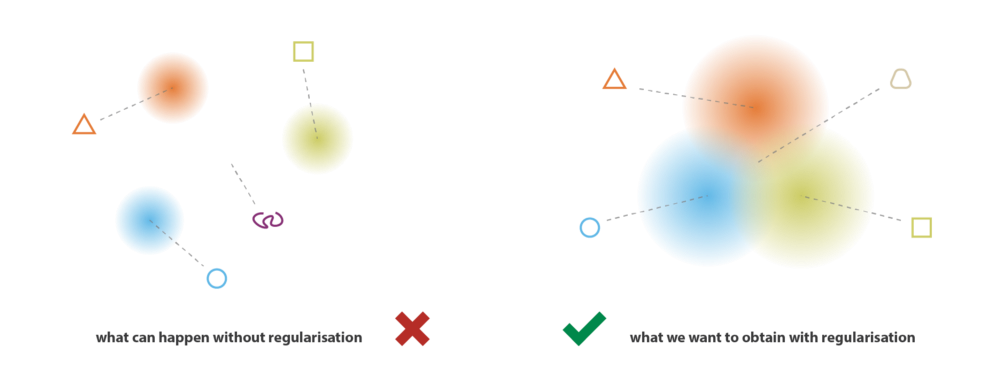
\includegraphics[width=16cm]{images/regularised_distributions_vae.png}
    \label{fig:regularised_distributions_vae}
\end{figure}
we have to regularise both the covariance matrix and the mean of the distributions
returned by the encoder. In practice, this regularisation is done by \textbf{enforcing
distributions to be close to a standard normal distribution}
\begin{figure}[H]
    \centering
    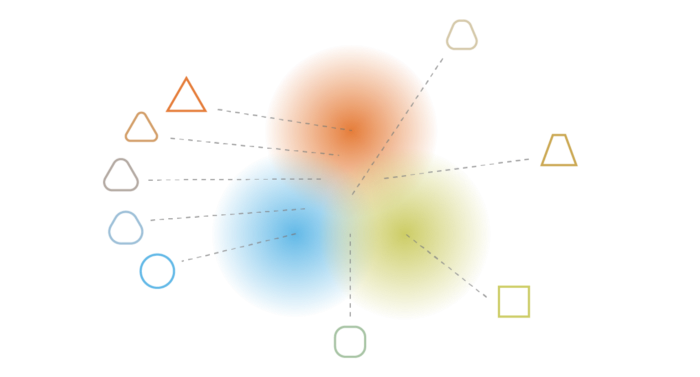
\includegraphics[width=12cm]{images/vae_regularisation.png}
    \label{fig:regularised_distributions_vae}
\end{figure}

\subsection{}

\subsection{贝叶斯混合高斯模型}


\section{Generative Adversarial Nets}

\subsection{Mode collapse}
https://aiden.nibali.org/blog/2017-01-18-mode-collapse-gans/

\subsection{Wasserstein GAN and the Kantorovich-Rubinstein Duality}
https://vincentherrmann.github.io/blog/wasserstein/

\subsection{vanila GAN}
$z \sim p(z) -> p_{data}(x)$
\begin{equation}
    \min_G \max_D V(D, G) = E_{\boldsymbol{x} \thicksim p_{data}(\boldsymbol{x})}[\log D(\boldsymbol{x})] + E_{\boldsymbol{z} \thicksim p_{\boldsymbol{z}}(\boldsymbol{z})}[\log (1 - D(G(\boldsymbol{z})))]
\end{equation}
The training criterion for the discriminator D, given any generator G, is to maximize the
quantity V(G, D)
\begin{equation}
    \begin{split}
        V(G, D) &= \int_{\boldsymbol{x}} p_{data}(\boldsymbol{x}) \log (D(\boldsymbol{x})) dx \int_{\boldsymbol{z}} p_{\boldsymbol{z}}(\boldsymbol{z}) \log(1 - D(g(\boldsymbol{z})))dz \\
        &= \int_{\boldsymbol{x}} p_{data}(\boldsymbol{x}) \log(D(\boldsymbol{x})) + p_g(\boldsymbol{x}) \log (1 - D(\boldsymbol{x})) dx
    \end{split}
\end{equation}

For any $(a, b) \in \mathbb{R}^2 \backslash {0, 0}$, the function $ y \to a\log(y) + b\log(1 - y)$
achieves its maximum in [0, 1] at $\frac{a}{a + b}$.
So, for G fixed, the optimal discriminator D is
\begin{equation}
    D_{G}^{*}(\boldsymbol{x}) = \frac{p_{data}(\boldsymbol{x})}{p_{data}(\boldsymbol{x}) + p_g(\boldsymbol{x})}
\end{equation}

Note that the training objective for D can be interpreted as maximizing the log-likelihood for
estimating the conditional probability $P(Y = y|\boldsymbol{x}), \boldsymbol{x} \in p_{data} or \in p_g$, then
\begin{equation}
    \begin{split}
        C(G) &= max_D V(G, D) \\
        &= \mathbb{E}_{\boldsymbol{x} \thicksim p_{data}}[\log D_G^*(\boldsymbol{x})] + \mathbb{E}_{\boldsymbol{z} \thicksim p_{\boldsymbol{z}}}[\log(1 - D_G^*(G(\boldsymbol{z})))] \\
        &= \mathbb{E}_{\boldsymbol{x} \thicksim p_{data}}[\log D_G^*(\boldsymbol{x})] + \mathbb{E}_{\boldsymbol{x} \thicksim p_{g}}[\log D_G^*(\boldsymbol{x})] \\
        &= \mathbb{E}_{\boldsymbol{x} \thicksim p_{data}}[\log \frac{p_{data}(\boldsymbol{x})}{p_{data}(\boldsymbol{x}) + p_g(\boldsymbol{x})}] + \mathbb{E}_{\boldsymbol{x} \thicksim p_g}[\log \frac{p_g(\boldsymbol{x})}{p_{data}(\boldsymbol{x}) + p_g(\boldsymbol{x})}]
    \end{split}
\end{equation}
The global minimum of C(G) is achieved if and onl if $p_g = p_{data}$. and
\begin{equation}
    C(G) = - \log 4
\end{equation}
and that by substracting this expression from $C(G) = V(D_G^*, G)$, we abtain:
\begin{equation}
    \begin{split}
        C(G) &= -log(4) + KL(p_{data}\| \frac{p_{data} + p_g}{2}) + KL(p_g \| \frac{p_data + p_g}{2}) \\
        &= -2\log(2) + 2JSD(p_{data}\|p_g)
    \end{split}
\end{equation}
在D最优的情况下,等价于优化JSD

\subsection{Latent space}
\begin{figure}[H]
    \centering
    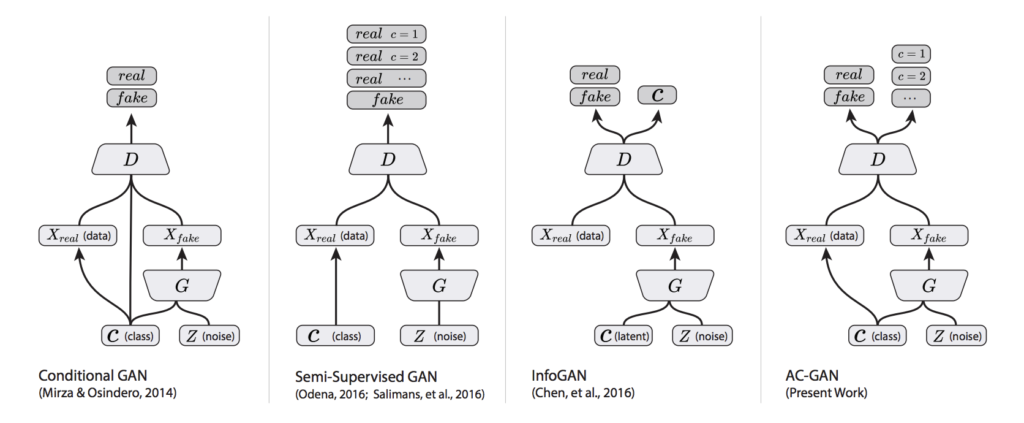
\includegraphics[width=16cm]{images/cgan_acgan.png}
    \label{fig:CGAN2ACGAN}
\end{figure}
\subsubsection{Conditional GAN}
使用辅助信息——label,将label和image绑定,分别输入到D和G中,
\begin{equation}
    \min_G \max_D V(D, G) = E_{\boldsymbol{x} \thicksim p_{data}(\boldsymbol{x})}[\log D(\boldsymbol{x}|\boldsymbol{y})] + E_{\boldsymbol{z} \thicksim p_{\boldsymbol{z}}(\boldsymbol{z})}[\log (1 - D(G(\boldsymbol{z}|\boldsymbol{y})))]
\end{equation}

\textbf{可以使用标签控制生成指定类型的图片}
\subsubsection{Semi-Supervised GAN}
\subsubsection{InfoGAN}
\subsubsection{ACGAN}

\subsection{Architecture}

\subsection{Object functions}

